\documentclass[12pt, a4paper]{report}
\usepackage[spanish]{babel}
\usepackage[utf8]{inputenc}
\usepackage{graphicx} 
\usepackage{amsmath}
\usepackage{algorithm}
\usepackage{hyperref}
\usepackage{xcolor}
\usepackage[noend]{algpseudocode}

\makeatletter
\def\BState{\State\hskip-\ALG@thistlm}
\makeatother

\graphicspath{ {images/} }

\hypersetup{
    colorlinks=true,
    linkcolor=black,
    urlcolor=blue
}

\title{%
\textbf{Simulación de Sistemas}\\
Trabajo Práctico 2: Autómata Celular Off-Lattice \\
\large \emph{Bandadas de Agentes Autopropulsados}
}

\author{Piñeiro, Eugenia Sol - 59449\\
Baiges, Matías Sebastián - 59076\\
Comerci Wolcanyik, Nicolás - 59520
}
\date{3 de septiembre de 2021}

\begin{document}

\maketitle

\tableofcontents
\newpage

\section{Introducción}
El objetivo del siguiente trabajo práctico es implementar un Autómata Celular \emph{Off-Latice}, 
a fin de analizar el comportamiento de partículas puntuales en base a distintos parámetros.\\

El autómata \emph{Off-Latice} se basa en un modelo matemático inspirado en el comportamiento colectivo de algunos Sistemas Naturales. Estos sujetos biológicos tienden a moverse con sus vecinos. Por ejemplo, bandadas, cardúmenes, manadas de cuadrúpedos o una colonia de bacterias.\cite{vicsek1995novel}\\

En cuanto al sistema, las partículas se desplazan con velocidad absoluta constante. Las mismas, en cada paso de tiempo, asumen el promedio de las direcciones de las partículas vecinas que se encuentran dentro de un radio \emph{r} con un ruido añadido de forma aleatoria.\\

Este modelo exhibe un comportamiento cooperativo entre las partículas, las cuales a medida que va avanzando el tiempo comienzan a moverse con una simetría de forma espontánea.\\ 

La evolución temporal de las partículas viene dada por las siguientes ecuaciones: 
\begin{equation}
\label{eq:velocity}
x_i(t+1) = x_i(t) + v_i(t) \Delta t 
\end{equation}

donde \emph{x} es la posición de la partícula, \emph{v} la velocidad, y $\Delta$\emph{t} el paso de tiempo.  

\begin{equation}
\label{eq:angle}
\theta _i(t+1) = \left\langle \theta _i(t)\right\rangle _r + \Delta \theta 
\end{equation}
donde $\Delta \theta  \epsilon  [-\frac{\eta}{2}; \frac{\eta}{2}]$ es el ruido añadido, siendo $\eta$ la amplitud del ruido, y \emph{$\left\langle \theta _i(t)\right\rangle _r$} es el promedio de los ángulos de todas las partículas en un radio \emph{r}.

\begin{equation}
\label{eq:avgangle}
\left\langle \theta _i(t)\right\rangle _r =  \frac{\left\langle sin(\theta _i(t))\right\rangle _r}{\left\langle cos(\theta _i(t))\right\rangle _r} 
\end{equation}

\section{Implementación}
La implementación del algoritmo \emph{Off-Lattice} se desarrolló en el lenguaje de programación \emph{Java}.\\

El flujo principal del programa (ver Figura \ref{fig:diagrama_flujo}) consiste en diversos pasos. En primer lugar, se obtienen los parámetros de configuración para iniciar la Simulación.\\

Luego, se generan partículas de forma aleatoria y se van actualizando tanto sus posiciones como sus ángulos con el algoritmo del autómata. \\

Por último, se guardan los resultados en distintos archivos que serán utilizados como \emph{input} para generar la Animación en \emph{Ovito} y realizar el postprocesamiento en \emph{Python} para hacer un análisis de resultados.\\

\begin{figure}[h]
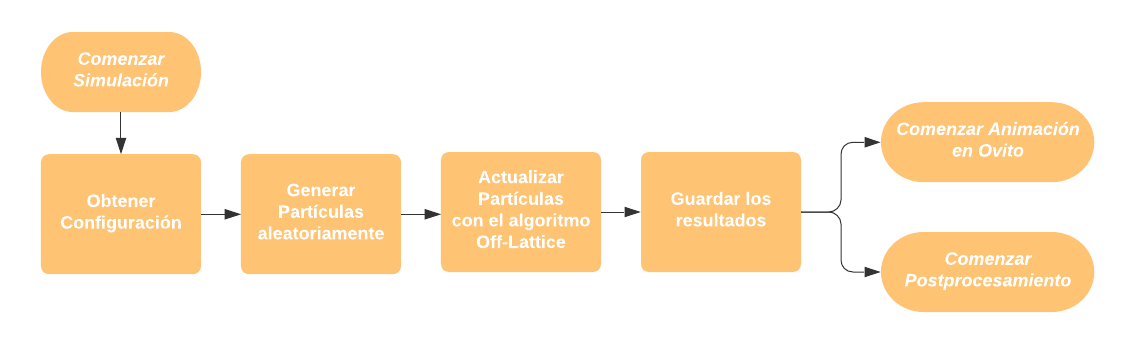
\includegraphics[scale=0.35]{Diagrama de flujo.png}
\centering 
\caption{Diagrama de Flujo}
\label{fig:diagrama_flujo}
\end{figure}

 
En cuanto a la implementación de la Simulación, se cuenta con distintas clases en Java (ver Figura \ref{fig:uml}). La clase que implementa el flujo principal (main) es \emph{OffLatticeSimulation}. Las partículas se modelaron con la clase \emph{VelocityPaticle}, que extiende de una clase \emph{Particle} y cuenta con su posición, ángulo y rapidez. Las mismas se generan a partir de la clase \emph{VelocityParticleGenerator}.\\

Para calcular la polarización de las mismas se cuenta con la clase \emph{Polarization}. El algoritmo del autómata se implementó en la clase \emph{OffLattice} que hace uso de las mencionadas anteriormente.\\  

A su vez, se cuenta con las clases para obtener los parámetros de configuración y obtención de resultados \emph{Config, XYZWriter, JsonWriter} y \emph{Postprocessing}, sobre las cuales no se entrará en detalle ya que corresponden al postprocesamiento.

\pagebreak

\begin{figure}[h]
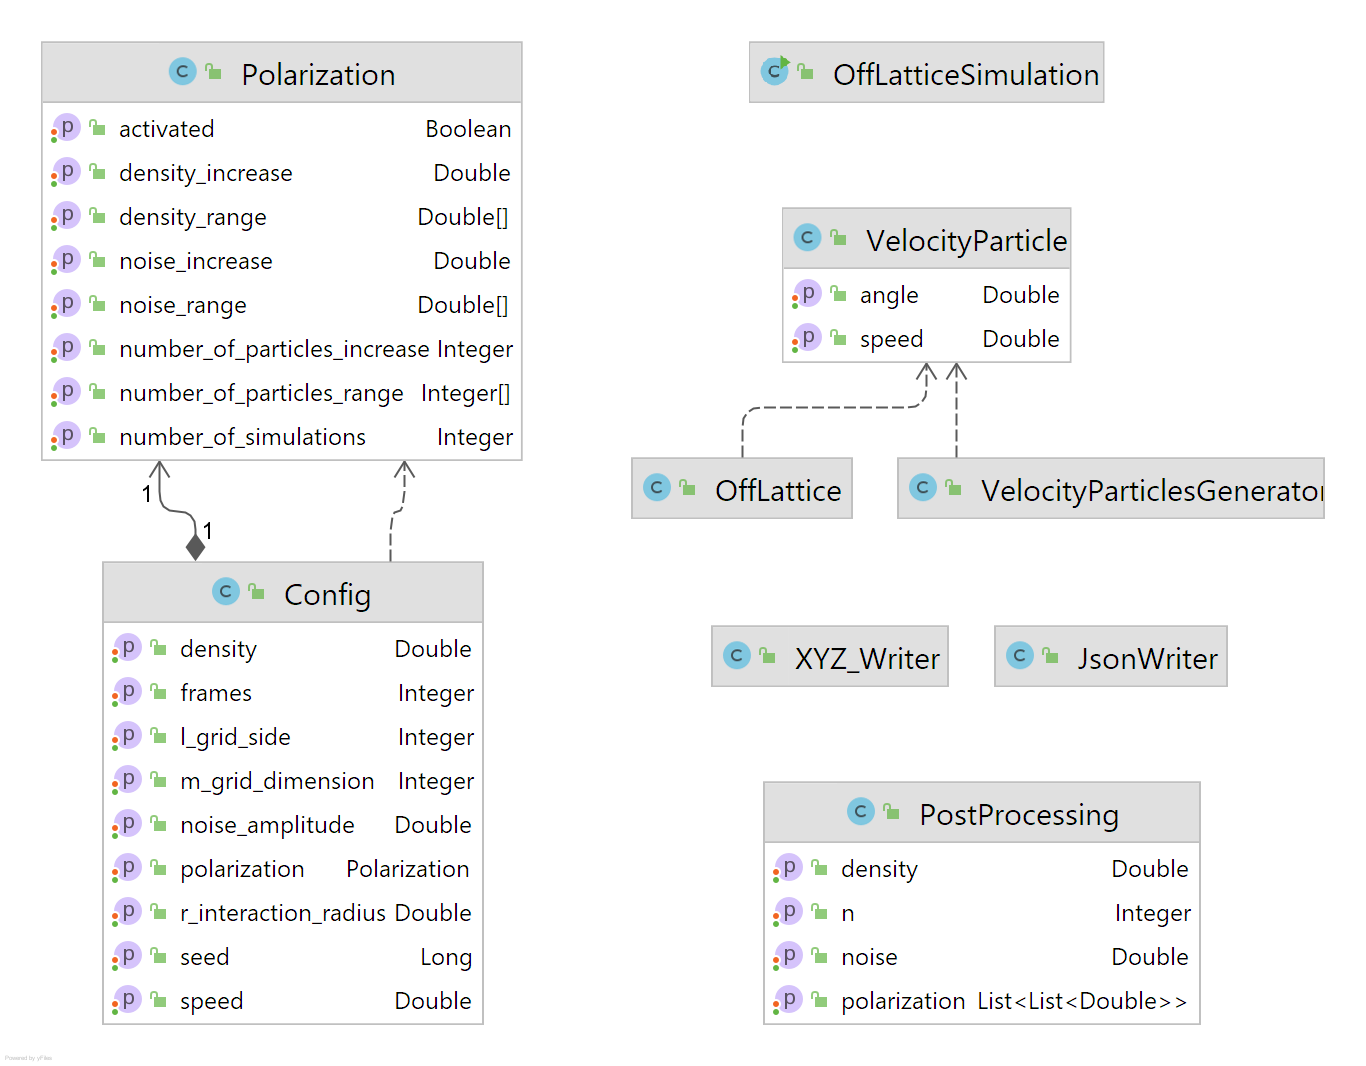
\includegraphics[scale=0.3]{UML.png}
\centering 
\caption{Diagrama UML}
\label{fig:uml}
\end{figure}

En el pseudocódigo correspondiente al flujo principal del programa (ver Algoritmo 1) se puede notar que se sigue el flujo mencionado previamente, en el cual se llama a la función \emph{readValues()} para obtener la configuración del sistema, luego se generan partículas de forma aleatoria invocando la función \emph{generateRandom()}, se llama al autómata Off-Lattice y por último se guardan los resultados en los archivos correspondientes.\\

En cuanto a la implementación del autómata (ver Algoritmo 2) cabe destacar que por cada pasa de tiempo (frame), en la línea 3 del pseudocódigo, se buscan los vecinos de las partículas a través del \emph{Cell Index Method}. Este método define una grilla de dimensión MxM y se utilizan condiciones de contorno periódicas \cite{cellIndex}.
Luego, se actualizan el ángulo y la posición de cada partícula utilizando las ecuaciones de Evolución Temporal (1) (2) y (3). 

\pagebreak
\begin{algorithm}
    \caption{Off-Lattice Simulation Main}\label{main}
    \begin{algorithmic}[1]
    \Procedure{main}{}
    \State $\textit{config} \gets \text{mapper.readValues()}$
    \State $particles \gets \textit{VelocityParticlesGenerator.generateRandom(config)}$
    \State $frames \gets \textit{OffLattice.simulate(config)}$
    \State $XYZ_Writer(FILENAME).addAllFrames(frames)$
    \EndProcedure
    \end{algorithmic}
\end{algorithm}
\begin{center}
Algoritmo 1. Flujo Principal del Programa
\end{center}

\begin{algorithm}
    \caption{Off-Lattice Algorithm}\label{offLattice}
    \begin{algorithmic}[1]
    \Procedure{simulate}{}
    \BState \emph{\textbf{for} frame in frames}:
    \State $\textit{neighbours} \gets \text{CellIndexMethod.search()}$
    \BState \emph{\textbf{for} particle in neighbours + itself}:
    \State $\textit{newAngle} \gets \text{atan2(sinAvg, cosAvg) + noise}$
    \State $particle.setAngle(newAngle)$
    \State $particle.setX((x + speed * cos(newAngle)) \ mod \  L)$
    \State $particle.setY((y + speed * sin(newAngle)) \ mod \ L)$
    \EndProcedure
    \end{algorithmic}
\end{algorithm}
\begin{center}
Algoritmo 2. Algoritmo del Autómata Off-Lattice
\end{center}

\section{Simulaciones}

El esquema del sistema (ver Figura \ref{fig:esquema}) consta de una grilla cuyos lados son de longitud \emph{L}, en la cual interactúan partículas con velocidad constante \emph{v} y radio de interacción \emph{r}.

\begin{figure}[h]
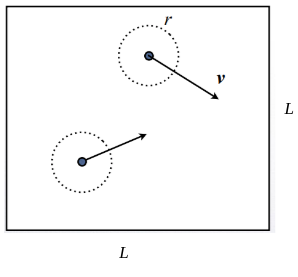
\includegraphics[scale=0.42]{esquema.png}
\centering 
\caption{Esquema del Sistema}
\label{fig:esquema}
\end{figure}

\pagebreak
Para realizar las simulaciones se utilizaron los siguientes parámentros: 
\begin{itemize}
    \item Radio de interacción entre partículas \emph{r = 1}
    \item Velocidad absoluta de las partículas \emph{v = 0.03}
    \item Amplitud del ruido \emph{$\eta$ $\epsilon$ [0; 2$\pi$]} 
    \item Lado de la grila L (Variable) 
    \item Cantidad de partículas N (Variable)
    \item Densidad $\rho = \frac{N}{L^2}$
    \item Cantidad de pasos \emph{frames} = 2000  
\end{itemize}

En cada simulación se observó la polarización del sistema, la cual se define con la siguiente ecuación: 
\begin{equation}
    \label{eq:polarization}
     v_a = \frac{1}{Nv} \left\lvert \sum_{i = 1}^{N} v_i \right\rvert
\end{equation}\\

Si la polarización tiende a cero, las partículas se encuentran en total desorden, mientras que si la polarización tiende a uno se dice que las partículas están polarizadas.\\

Para correr las simulaciones se utilizarán las siguientes configuraciones: 
\begin{enumerate}
    \item Para analizar el ruido se utilizó N=300, $\rho$=0.6 y $\eta$ variable
    \item Para analizar la densidad se utilizó N=300, $\eta$=0.8 y $\rho$ varibale 
    \item Densidad y ruido pequeños:  N = 300, L = 25, ($\rho$ = 0.48), $\eta$ = 0.1
    \item Densidad y ruido grandes:  N = 300, L = 7, ($\rho$ = 6.12), $\eta$ = 2.0  
    \item Densidad grande y ruido pequeño: N = 300,	L = 5, ($\rho$ = 12), $\eta$ = 0.1
\end{enumerate}


\section{Resultados}

% A partir de las configuraciones mencionadas previamente, se obtuvieron los siguientes resultados tras analizar el efecto del ruido y la densidad.

\subsection{Análisis del Ruido}

Luego de realizar simulaciones bajo las configuraciones propuestas (ver Figuras \ref{fig:noise_N300_d06_n05}, \ref{fig:noise_N300_d06_n1_5} y \ref{fig:noise_N300_d06_n5}), se observó que a medida que el ruido aumentaba, las particulas tendían a dispersarse, dirigiendose hacia distintas direcciones, es decir, manteniendo la cantidad de partículas y el ruido constante, \emph{al aumentar el ruido, la polarización disminuye}.\\

En caso de poco ruido (ver Figura \ref{fig:noise_N300_d06_n05}), se pudo observar como las partículas al cabo de un par de pasos (\emph{frames}) se movían en la misma dirección (\emph{partículas altamente polarizadas}).\\

Al aumentar el ruido (ver Figura \ref{fig:noise_N300_d06_n1_5}), se observó que no se llegaba a una polarización tan clara como en el caso anterior, formándose grupos representados a través de los distintos colores.\\

Finalmente para $\eta = 5$ (ver Figura \ref{fig:noise_N300_d06_n5}), se obtuvo una imágen invariable de múltiples colores y desorden a través de toda la simulación.

\begin{figure}[h]
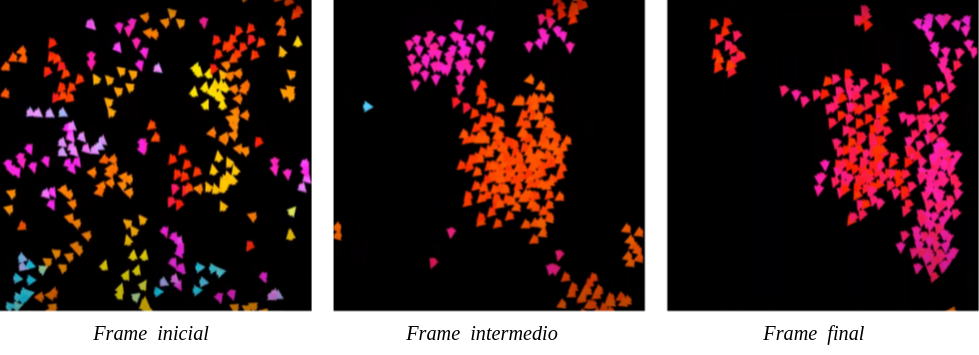
\includegraphics[scale=0.4]{noise_N300_d06_n05.png}
\centering 
\caption{Capturas de los frames inicial, intermedio y final de una Animación con N=300; $\rho$=0.6 y $\eta$=0.5 \href{https://www.youtube.com/watch?v=hD-HLrDGDrI}{\underline{Ver Animación}}} 
\label{fig:noise_N300_d06_n05}
\end{figure}

\begin{figure}[h]
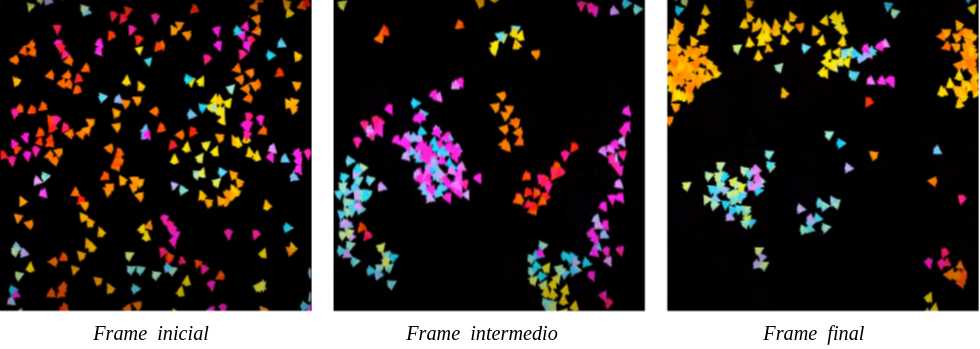
\includegraphics[scale=0.4]{noise_N300_d06_n1_5.png}
\centering 
\caption{Capturas de los frames inicial, intermedio y final de una Animación con N=300; $\rho$=0.6 y $\eta$=1.5 \href{https://www.youtube.com/watch?v=pNaZWqdfaxg}{\underline{Ver Animación}}} 
\label{fig:noise_N300_d06_n1_5}
\end{figure}

\pagebreak
\begin{figure}[h]
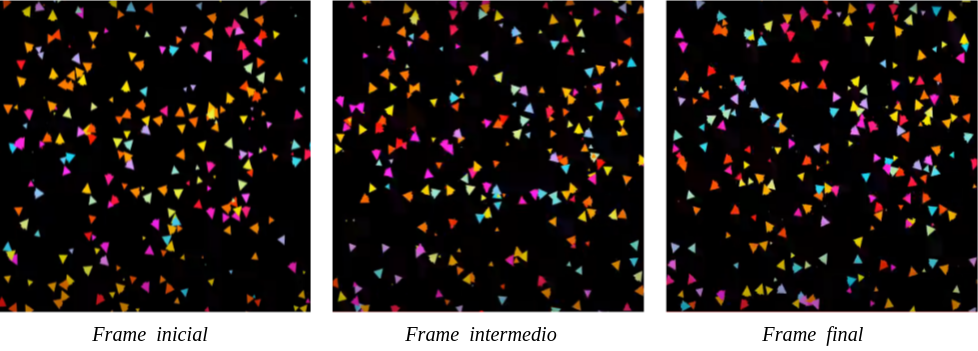
\includegraphics[scale=0.4]{noise_N300_d06_n5.png}
\centering 
\caption{Capturas de los frames inicial, intermedio y final de una Animación con N=300; $\rho$=0.6 y $\eta$=5 \href{https://www.youtube.com/watch?v=KpLdzP7WLP8}{\underline{Ver Animación}}}
\label{fig:noise_N300_d06_n5}
\end{figure}

También se observó este mismo fenómeno al comparar la evolución de la polarización en función del tiempo para distintos valores de ruidos (ver Figura \ref{fig:noise_pola_vs_time_multiple_n}). \\

Además, se pudo ver esta situación para distintos valores de ruido (ver Figura \ref{fig:pola_vs_noise}), y para distintas cantidades de partículas (ver Figura \ref{fig:pola_vs_noise_multiple_n}), donde vimos que mientras menos partículas, mayor era la polarización manteniendo el ruido constante.

\pagebreak
\begin{figure}[h]
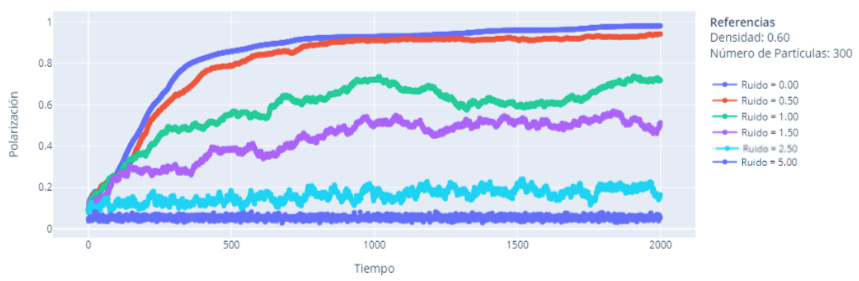
\includegraphics[scale=0.45]{noise_pola_vs_time_multiple_n.png}
\centering 
\caption{Polarización en función del tiempo para múltiples valores del ruido, $\rho$=0.6, N=300 }
\label{fig:noise_pola_vs_time_multiple_n}
\end{figure}

\begin{figure}[h!]
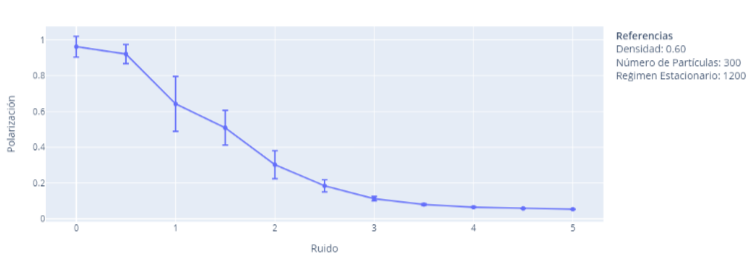
\includegraphics[scale=0.5]{pola_vs_noise.png}
\centering 
\caption{Polarización en función del ruido para $\rho$=0.6, N=300 y considerando el frame 1200 como comienzo del régimen estacionario.}
\label{fig:pola_vs_noise}
\end{figure}
 
\begin{figure}[h!]
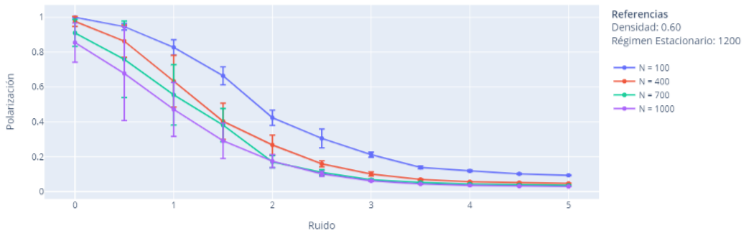
\includegraphics[scale=0.5]{pola_vs_noise_multiple_n.png}
\centering 
\caption{Polarización en función del ruido para múltiples valores de N con $\rho$=0.6 y considerando el frame 1200 como comienzo del régimen estacionario.}
\label{fig:pola_vs_noise_multiple_n}
\end{figure}

\subsection{Análisis de la Densidad}

Luego de realizar simulaciones bajo las configuraciones propuestas (ver Figuras \ref{fig:density_N300_n08_d025}, \ref{fig:density_N300_n08_d3} y \ref{fig:density_N300_n08_d6}), se observó que a medida que se aumentaba la densidad de partículas, las partículas tienden a moverse de manera más ordenada, es decir, manteniendo la cantidad de partículas y el ruido constantes, \emph{al aumentar la densidad de partículas, la polarización aumenta}.\\

En particular, para un densidad muy pequeña (ver Figura \ref{fig:density_N300_n08_d025}) se notó que las partículas comenzaban dispersas y luego de un tiempo se dividían en grupos. Dentro de cada uno de los grupos todas las partículas se desplazaban en la misma dirección. \\

En cambio, tomando un valor de densidad intermedio (ver Figura \ref{fig:density_N300_n08_d3}) se observó que las partículas al principio generaban pequeños grupos pero luego comenzaban a desplazarse todas en las mismas dirección.\\

Por último, tomando un valor de densidad grande (ver Figura \ref{fig:density_N300_n08_d6}) se pudo notar que rápidamente las partículas se acomodaban en la misma dirección. 

\begin{figure}[h]
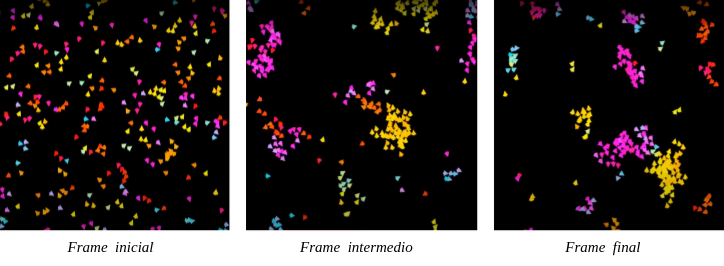
\includegraphics[scale=0.54]{density_N300_n08_d025.png}
\centering 
\caption{Capturas de los frames inicial, intermedio y final de una Animación con N=300; $\rho$=0.25 y $\eta$=0.8 \href{https://www.youtube.com/watch?v=j0crtCYmx9E}{\underline{Ver Animación}}}
\label{fig:density_N300_n08_d025}
\end{figure}

\begin{figure}[h]
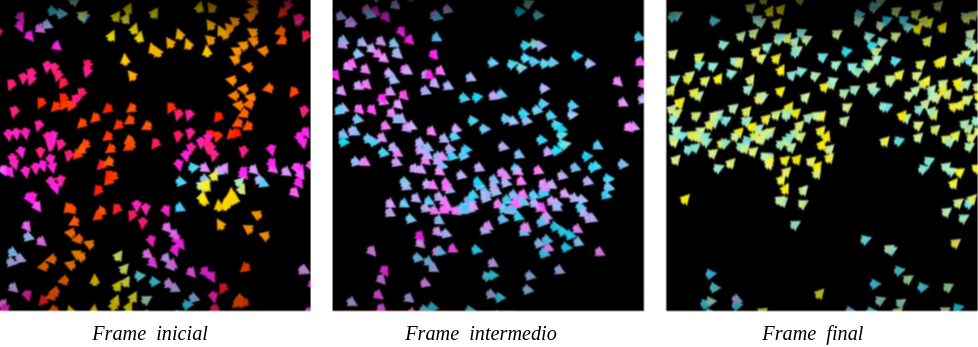
\includegraphics[scale=0.4]{density_N300_n08_d3.png}
\centering 
\caption{Capturas de los frames inicial, intermedio y final de una Animación con N=300; $\rho$=3 y $\eta$=0.8 \href{https://www.youtube.com/watch?v=Ez3LWEwRvmk}{\underline{Ver Animación}}}
\label{fig:density_N300_n08_d3}
\end{figure}

\pagebreak
\begin{figure}[h]
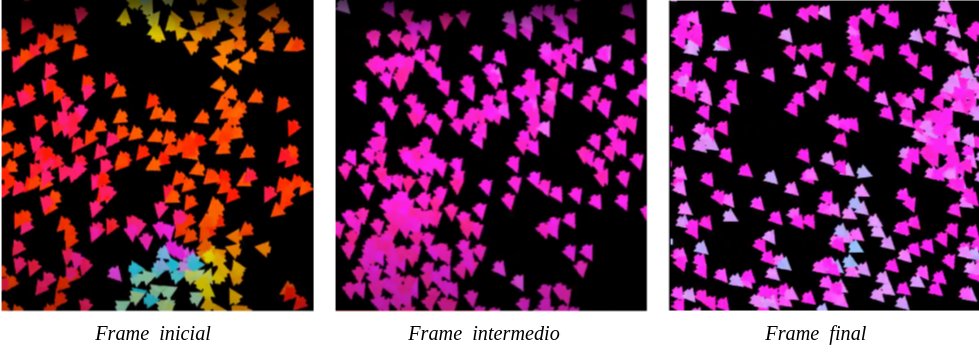
\includegraphics[scale=0.4]{density_N300_n08_d6.png}
\centering 
\caption{Capturas de los frames inicial, intermedio y final de una Animación con N=300; $\rho$=6 y $\eta$=0.8 \href{https://www.youtube.com/watch?v=t88TD__ushc}{\underline{Ver Animación}}} % TODO CAMBIAR LINK 
\label{fig:density_N300_n08_d6}
\end{figure}

Analizando la polarización en función del tiempo para múltiples valores de densidad, dejando el resto de los parámetros constantes (ver Figura \ref{fig:density_pola_vs_time}), se puede apreciar que a medida que se aumentan los valores de densidad, aumenta la polarización a lo largo del tiempo. Esto se corresponde con lo mencionado previamente sobre las partículas alineandose (aumenta la polarización) a medida que aumenta la densidad.\\

Cabe destacar que mientras más bajo es el valor de la densidad, se notó que se necesitaban más frames para alcanzar un régimen estacionario. En este caso se decidió promediar los valores de polarización a partir del frame 1200 para graficar la polarización en función de la densidad para un ruido determinado (ver Figura \ref{fig:pola_vs_density}) debido a que aproximadamente a partir de allí los valores de polarización son similares.\\


\begin{figure}[h]
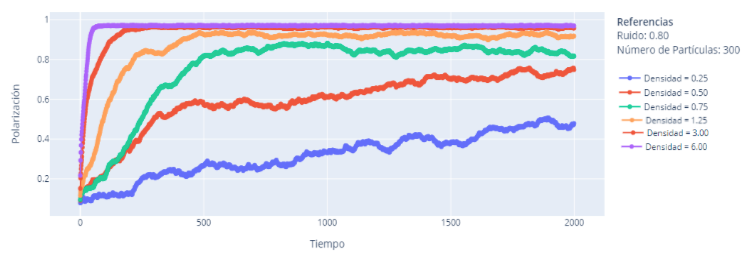
\includegraphics[scale=0.5]{density_pola_vs_time.png}
\centering 
\caption{Polarización en función del tiempo para múltiples valores de densidad con N=300; $\eta$=0.8}
\label{fig:density_pola_vs_time}
\end{figure}

% \pagebreak
\begin{figure}[h]
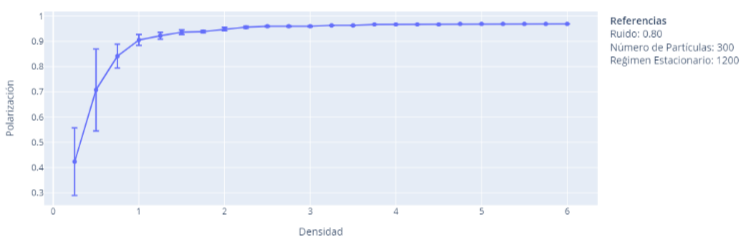
\includegraphics[scale=0.5]{pola_vs_density.png}
\centering 
\caption{Polarización en función de la densidad con N=300; $\eta$=0.8 usando el frame 1200 como comienzo del régimen estacionario.}
\label{fig:pola_vs_density}
\end{figure}

\subsection{Comportamientos Destacados}

Se utilizaron distintas configuraciones propuestas en el paper \cite{vicsek1995novel} con el objetivo de evaluar distintos comportamientos destacados del sistema.\\

En primer lugar, se utilizaron valores de densidad y ruido pequeños y se pudo notar que las partículas tienden a formar grupos moviendose de forma coherente en direcciones aleatorias (ver Figura \ref{fig:d_n_small})\\  

Luego, para valores de densidad y ruido grandes (ver Figura \ref{fig:d_n_big}) se notó que las partículas se desplazan de forma aleatoria pero con cierta correlación.\\

Por último, con una densidad grande y un ruido pequeño (ver Figura \ref{fig:d_big_n_small}) se notó que el movimiento se vuelve ordenado para todas las partículas.
 
\begin{figure}[h]
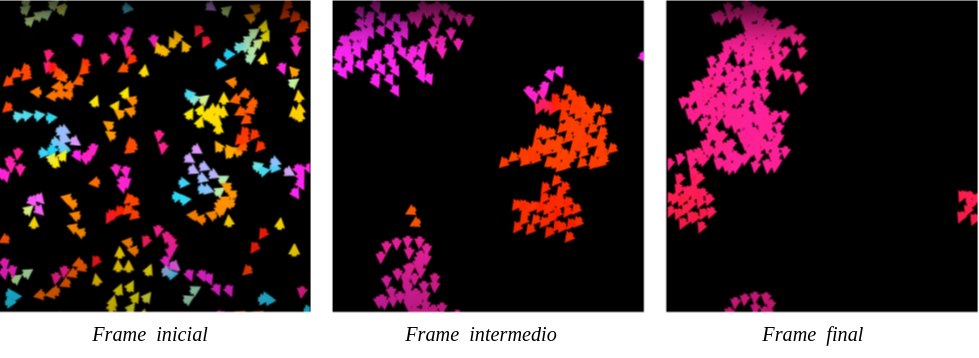
\includegraphics[scale=0.4]{d_n_small.png}
\centering 
\caption{Capturas de los frames inicial, intermedio y final de una Animación con  N = 300; L = 25;	($\rho$ = 0.48); $\eta$ = 0.1 \href{https://www.youtube.com/watch?v=V2oRjjUPpmY}{\underline{Ver Animación}}} 
\label{fig:d_n_small}
\end{figure}


\begin{figure}[h]
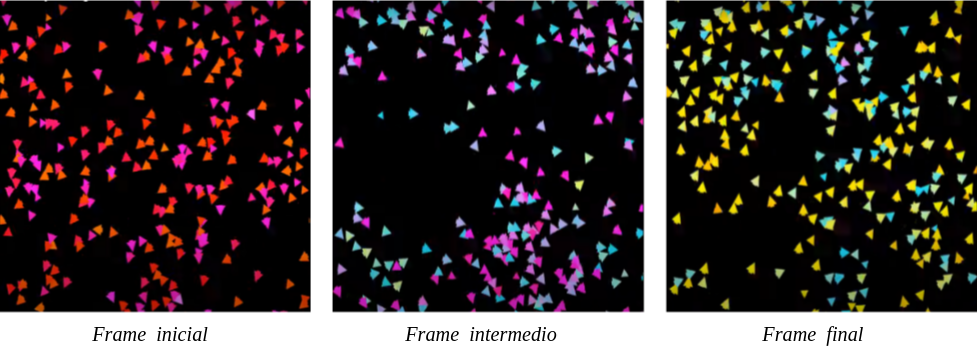
\includegraphics[scale=0.4]{d_n_big.png}
\centering 
\caption{Capturas de los frames inicial, intermedio y final de una Animación con N = 300; L = 7; ($\rho$ = 6.12); $\eta$ = 2.0 \href{https://www.youtube.com/watch?v=t88TD__ushc}{\underline{Ver Animación}}} 
\label{fig:d_n_big}
\end{figure}

\pagebreak
\begin{figure}[h]
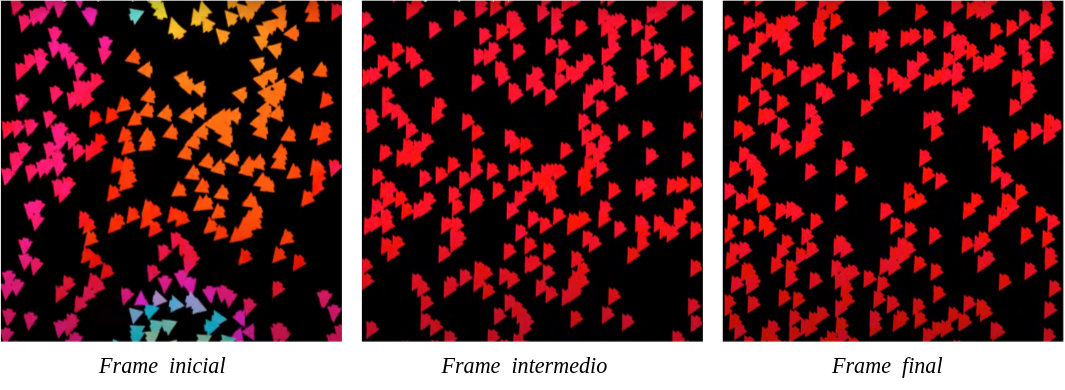
\includegraphics[scale=0.4]{d_big_n_small.png}
\centering 
\caption{Capturas de los frames inicial, intermedio y final de una Animación con N = 300; L = 5; ($\rho$ = 12); $\eta$ = 0.1  \href{https://www.youtube.com/watch?v=CnaNaZNd1MY}{\underline{Ver Animación}}} 
\label{fig:d_big_n_small}
\end{figure}

\section{Conclusiones}
Teniendo en cuenta los resultados obtenidos a partir de las simulaciones, se llegó a las siguientes conclusiones:
\begin{itemize}
    \item Manteniendo la cantidad de partículas y la densidad constantes, al aumentar el ruido disminuye la polarización.
    \item Manteniendo la cantidad de partículas y el ruido constantes, al aumentar la densidad de partículas aumenta la polarización.
    \item El sistema presenta distintos comportamientos según los parámetros elegidos.
\end{itemize}

\bibliographystyle{plain}
\bibliography{references}

\end{document}